
\section{Effectiveness of PLink Collectives}
We evaluate the effectiveness of \cmpi with a series of microbenchmarks from various communication backends and real-world applications that uses \collectives algorithms. We represent speedup by comparing the performance we get from the best rank ordering and worst rank ordering. We opt to avoid comparing with the original rank ordering because it is random, and has a wide performance distribution (Figure~\ref{fig:azringperformance}).

\subsection{Experimental Setup}
Our experiments are conducted on two public clouds, \azure and \ectwo. We enable network acceleration on both clouds, and set TCP congestion control protocol to DCTCP. We include microbenchmarks that exercise ring, having doubling, double binary tree and bcube algorithms.  All experiments run on Ubuntu 19 with kernel 5. We mainly focus our evaluation on one of the most important \collectives tasks, \textit{allreduce} for its popularity and generality. %We use unmodified Facebook Gloo~\cite{glooalgo70:online}, OSU MPI microbenchmark~\cite{10.1007/978-3-642-33518-1_16} and Nvidia NCCL~\cite{NVIDIACo76:online} with OpenMPI 4. We use lightgbm~\cite{Ke2017LightGBMAH} to evaluate the real-world impact of \cmpi. 

\subsection{Prediction Accuracy of Cost Model}
While the goal of the cost model is not to predict the actual performance, but rather, it should preserve the relative order of performance, i.e., $p_{pred}(\mathbb{R}_1) < p_{pred}(\mathbb{R}_2) \implies p_{real}(\mathbb{R}_1) < p_{real}(\mathbb{R}_2)$ should hold true for as many pairs of $(R_i, R_j)$s as possible. Because our optimization goal is a lower cost value. We demonstrate this for ring based \mpi algorithms by generating 10 different rank orders, with the $i$-th order approximately corresponds to the $10i$-th percentile in the range of costs found by the solver. We obtain performance data for Facebook Gloo and OpenMPI running OSU Benchmark on 64 F16 nodes on \azure and 64 C5 nodes on \ectwo. We then compute Spearman~\cite{spearman} correlation coefficient between the predicted performance and the actual performance for each setup~(Table~\ref{table:correlation}). 

\begin{table}[t!]
	\centering
	\footnotesize
	\begin{tabular}{|c|c|c|}
		\hline 
	    Setup & Azure & EC2  \\
		\hline
		Gloo Ring 100MB      & 0.58 & 0.78  \\
		\hline
		OpenMPI Ring 100MB      & 0.81 & 0.94 \\
		\hline
	\end{tabular}
	\caption{Spearman correlation coefficient between predicted performance from cost model and actual performance.}
	\label{table:correlation}
\end{table}

%Figure~\ref{fig:azringperformance} shows where the predicted best (purple dotted line) and worst performance (black dotted line) using the cost model landed in the performance distribution from 500 random ordering: the $\mathbb{R}$ that is predicted to achieve worst/best performance falls in the 99th/1st percentile of the total observed distribution. While not perfect, we believe this is acceptable due to the imperfection of the cost model and limitation of solvers. 

\subsection{Microbenchmark Performance}
We now evaluate \cmpi{}'s efficacy with microbenchmarks of \mpi algorithms introduced earlier. We report mean speedup of 20 iterations. We run all benchmarks with 512 F16 nodes on \azure, except for NCCL, which runs on 64 P3.8xLarge GPU nodes on \ectwo. Particularly, we set $B=4$ for BCube; for NCCL, we use a single binary tree reduction for small buffers, and ring for large buffers. In all benchmarks we reduce a buffer of 100MB, except for Nvidia NCCL, where we reduce a small buffer of 4B to trigger the tree algorithm.


\begin{figure}[t!]
	\centering
	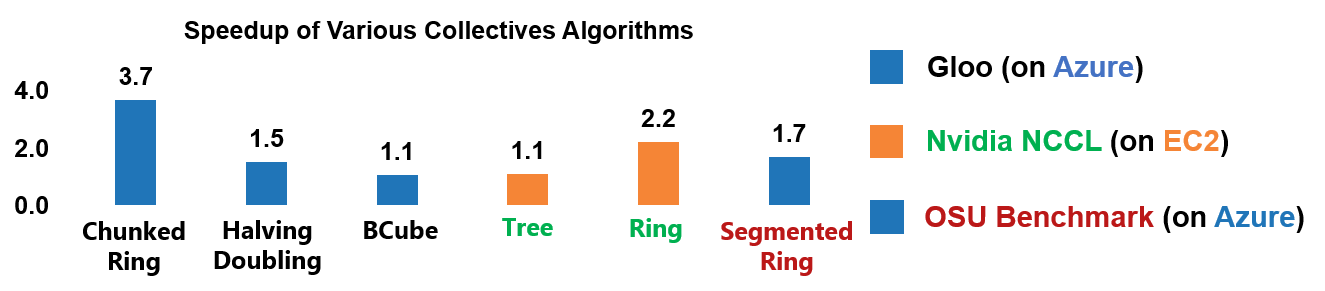
\includegraphics[width=.6\linewidth]{Figures/collectivesperformance.png}
	\caption{Speedups achieved by just using the rank ordering produced by our tool in various \collectives algorithms across multiple distributed communication backends at a large scale.}
	\label{fig:collectivesPerformance}
\end{figure}

Figure~\ref{fig:collectivesPerformance} shows a summary of speedups achieved using \cmpi on these benchmarks, ranging from 1.1x-3.7x, with the ring-family algorithms benefiting the most. We speculate the reason for the effectiveness is that they have a much wider performance distribution, as each permutation of the order can potentially generate a different performance (cost of each hop is on the critical path); they also have simpler cost model, allowing the solvers to quickly navigate the objective landscape. On the other hand, halving doubling, BCube and tree algorithms have complex objectives -- sum of maximums, resulting in a narrower performance distribution because mutation of the ordering may not change the cost at all if the mutation does not cause critical path to change. %This adds to difficulty of minimizing the objectives, because the solver itself relies on efficiently generating new cost values to proceed. 

\subsection{End-to-end Performance Impact on Real-world Applications}
\noindent \textbf{Speedup Distributed Gradient Boosted Decision Tree Training}. We evaluate \cmpi{}'s impact on LightGBM~\cite{Ke2017LightGBMAH}, a gradient boosted decision tree training system. We use data parallelism to run \textit{lambdarank} with metric \textit{ndcg}. Communication-wise, this workload runs two \collectives tasks: \textit{allreduce} and \textit{reducescatter}. %Each call to \textit{allreduce} reduces 24B of data, and approximately 1KB for \textit{reducescatter}. 
These two tasks are called sequentially when considering all tree leaves for split in each iteration, resulting in very frequent invocations. At our scale of 512 nodes, LightGBM automatically chooses to use halving and doubling for both \textit{reducescatter} and \textit{allreduce}. We use a typical dataset that represents an actual workload in our organization with 5K columns and a total size of 10GB for each node. We train 1000 trees, each with 120 leaves. We exclude the time it takes to load data from disk to memory, and report average speedup of 1000 iterations. \cmpi generated rank ordering speeds up training by 1.3x.

\noindent \textbf{Speedup Distributed Deep Neural Network Training}. We show \cmpi{}'s effectiveness on distributed training of DNNs with Caffe2/Pytorch, on 64 EC2 p3.8xLarge nodes with data parallelism and batch size of 64/GPU. We train AlexNet on ImageNet dataset. Since our \cmpi{} does not change computation and only improves communication efficiency of the \textit{allreduce} operation at iteration boundary, we report speedup of training in terms of images/second, averaged across 50 iterations. We use the ring chunked algorithm which achieves the best baseline performance, and the \cmpi{}-optimized rank ordering of VM nodes achieves a speedup of 1.2x.

